\documentclass{article} % For LaTeX2e
\usepackage{iclr2026_conference,times}

% Optional math commands from https://github.com/goodfeli/dlbook_notation.
\input{math_commands.tex}

\usepackage{hyperref}
\usepackage{url}
\usepackage{graphicx}
\usepackage{booktabs}
\usepackage{tabularx}
\usepackage{multirow}
\usepackage{amsmath,amssymb}

\title{StealthRL: Reinforcement Learning Paraphrase Attacks for\\
Multi-Detector Evasion of AI-Text Detectors}

\author{Anonymous Authors}

% \iclrfinalcopy % Uncomment for camera-ready version, but NOT for submission.
\begin{document}

\maketitle

\begin{abstract}
We introduce \emph{StealthRL}, a reinforcement-learning framework that paraphrases AI-generated text to evade detection while preserving meaning and fluency, enabling systematic red-teaming of AI-text detectors. The challenge is to reduce detector confidence at strict low-FPR operating points without collapsing semantic fidelity or overfitting to a single detector family. StealthRL fine-tunes a single Qwen3-4B paraphraser with LoRA \cite{hu2021loralowrankadaptationlarge} and a multi-objective reward combining detector evasion, semantic similarity, and fluency. On the MAGE benchmark with three detectors (RoBERTa OpenAI, Fast-DetectGPT, Binoculars), StealthRL reduces mean TPR@1\%FPR from 0.27 (no attack) to 0.04 while maintaining high semantic similarity (0.953 E5 cosine), outperforming simple paraphrasing and a detector-guided baseline. We release an anonymized code package in the supplementary material with a placeholder anonymous link for reproducibility.
\end{abstract}

\section{Introduction}
AI-generated text detectors are widely deployed in academic integrity, content moderation, and misinformation pipelines, yet their robustness to paraphrasing remains brittle. Recent work shows that detector performance can drop sharply under paraphrase attacks, motivating adversarial evaluation and red-teaming rather than static benchmarking. We focus on the adversarial aspect: how to generate high-fidelity paraphrases that reliably evade multiple detector families, while maintaining readability and semantic fidelity.

We present \textbf{StealthRL}, a reinforcement-learning paraphraser trained to reduce detector confidence under a strict low-FPR operating point. StealthRL is designed to (i) train against multiple detector families to promote transfer, (ii) preserve semantic content and fluency via auxiliary reward terms, and (iii) provide an evaluation harness that reports transfer and attack success at 1\% FPR. We position StealthRL as a red-teaming tool that helps stress-test detector robustness and guide defensive improvements.

\paragraph{Contributions.}
\begin{itemize}
  \item \textbf{Multi-detector RL paraphrasing.} We train a single paraphrase policy against a detector ensemble using group-relative policy optimization with LoRA, enabling efficient adversarial fine-tuning.
  \item \textbf{Low-FPR evaluation protocol.} We report attack success across multiple detector families at TPR@1\%FPR and release an evaluation pipeline that produces heatmaps and tradeoff curves.
  \item \textbf{Empirical results.} On MAGE, StealthRL reduces mean TPR@1\%FPR to 0.04 (from 0.27 for no attack) while maintaining high semantic similarity.
\end{itemize}

\paragraph{Anonymized code release.}
An anonymized code release containing training and evaluation scripts is included in the supplementary material. A placeholder anonymous link is provided: \url{https://anonymous.4open.science/r/STEALTHRL}.

\section{Related Work}
Detector families include curvature-based methods (DetectGPT and Fast-DetectGPT) and paired-LM detectors such as Binoculars. \cite{mitchell2023detectgptzeroshotmachinegeneratedtext,bao2024fastdetectgptefficientzeroshotdetection,hans2024spottingllmsbinocularszeroshot} Recent evasion work focuses on paraphrase attacks and RL-based humanization, including Adversarial Paraphrasing and AuthorMist, while character-level attacks such as homoglyph substitution demonstrate strong but often less readable perturbations. \cite{cheng2025adversarialparaphrasinguniversalattack,david2025authormistevadingaitext,creo2025silverspeakevadingaigeneratedtext} StealthRL builds on these directions by training a single paraphrase policy against a detector ensemble and evaluating transfer at strict low-FPR operating points.

\section{Threat Model}
We assume \textbf{black-box access to detector scores}, i.e., the attacker can query detector confidence but does not require gradients. In practice, detectors are often open-source or deployed with a confidence API, so both black-box scoring and open-source replication are realistic. We evaluate transfer to a held-out detector family to test robustness beyond the training ensemble.

\section{Method}
Given AI-generated text $x$, we learn a paraphrase policy $\pi_\theta(y\mid x)$ that produces $y$ with low detector confidence while preserving meaning and fluency. We optimize a composite reward:
\begin{equation}
R(x,y) = \alpha R_{\text{det}}(y) + \beta R_{\text{sem}}(x,y) + \gamma R_{\text{ppl}}(y),
\end{equation}
where $R_{\text{det}}$ is the ensemble detector score (lower AI probability), $R_{\text{sem}}$ is E5 embedding cosine similarity, and $R_{\text{ppl}}$ is a fluency proxy derived from a frozen LM. We train with group-relative policy optimization (GRPO) and LoRA adapters \cite{hu2021loralowrankadaptationlarge} on Qwen/Qwen3-4B-Instruct-2507 (rank 32, $\alpha=32$, dropout 0.05). Training uses group size 4, learning rate $2.8\\times10^{-4}$, batch size 16, and two epochs. The detector ensemble used for training is RoBERTa OpenAI + Fast-DetectGPT with weights 0.6/0.4.

\begin{figure}[t]
  \centering
  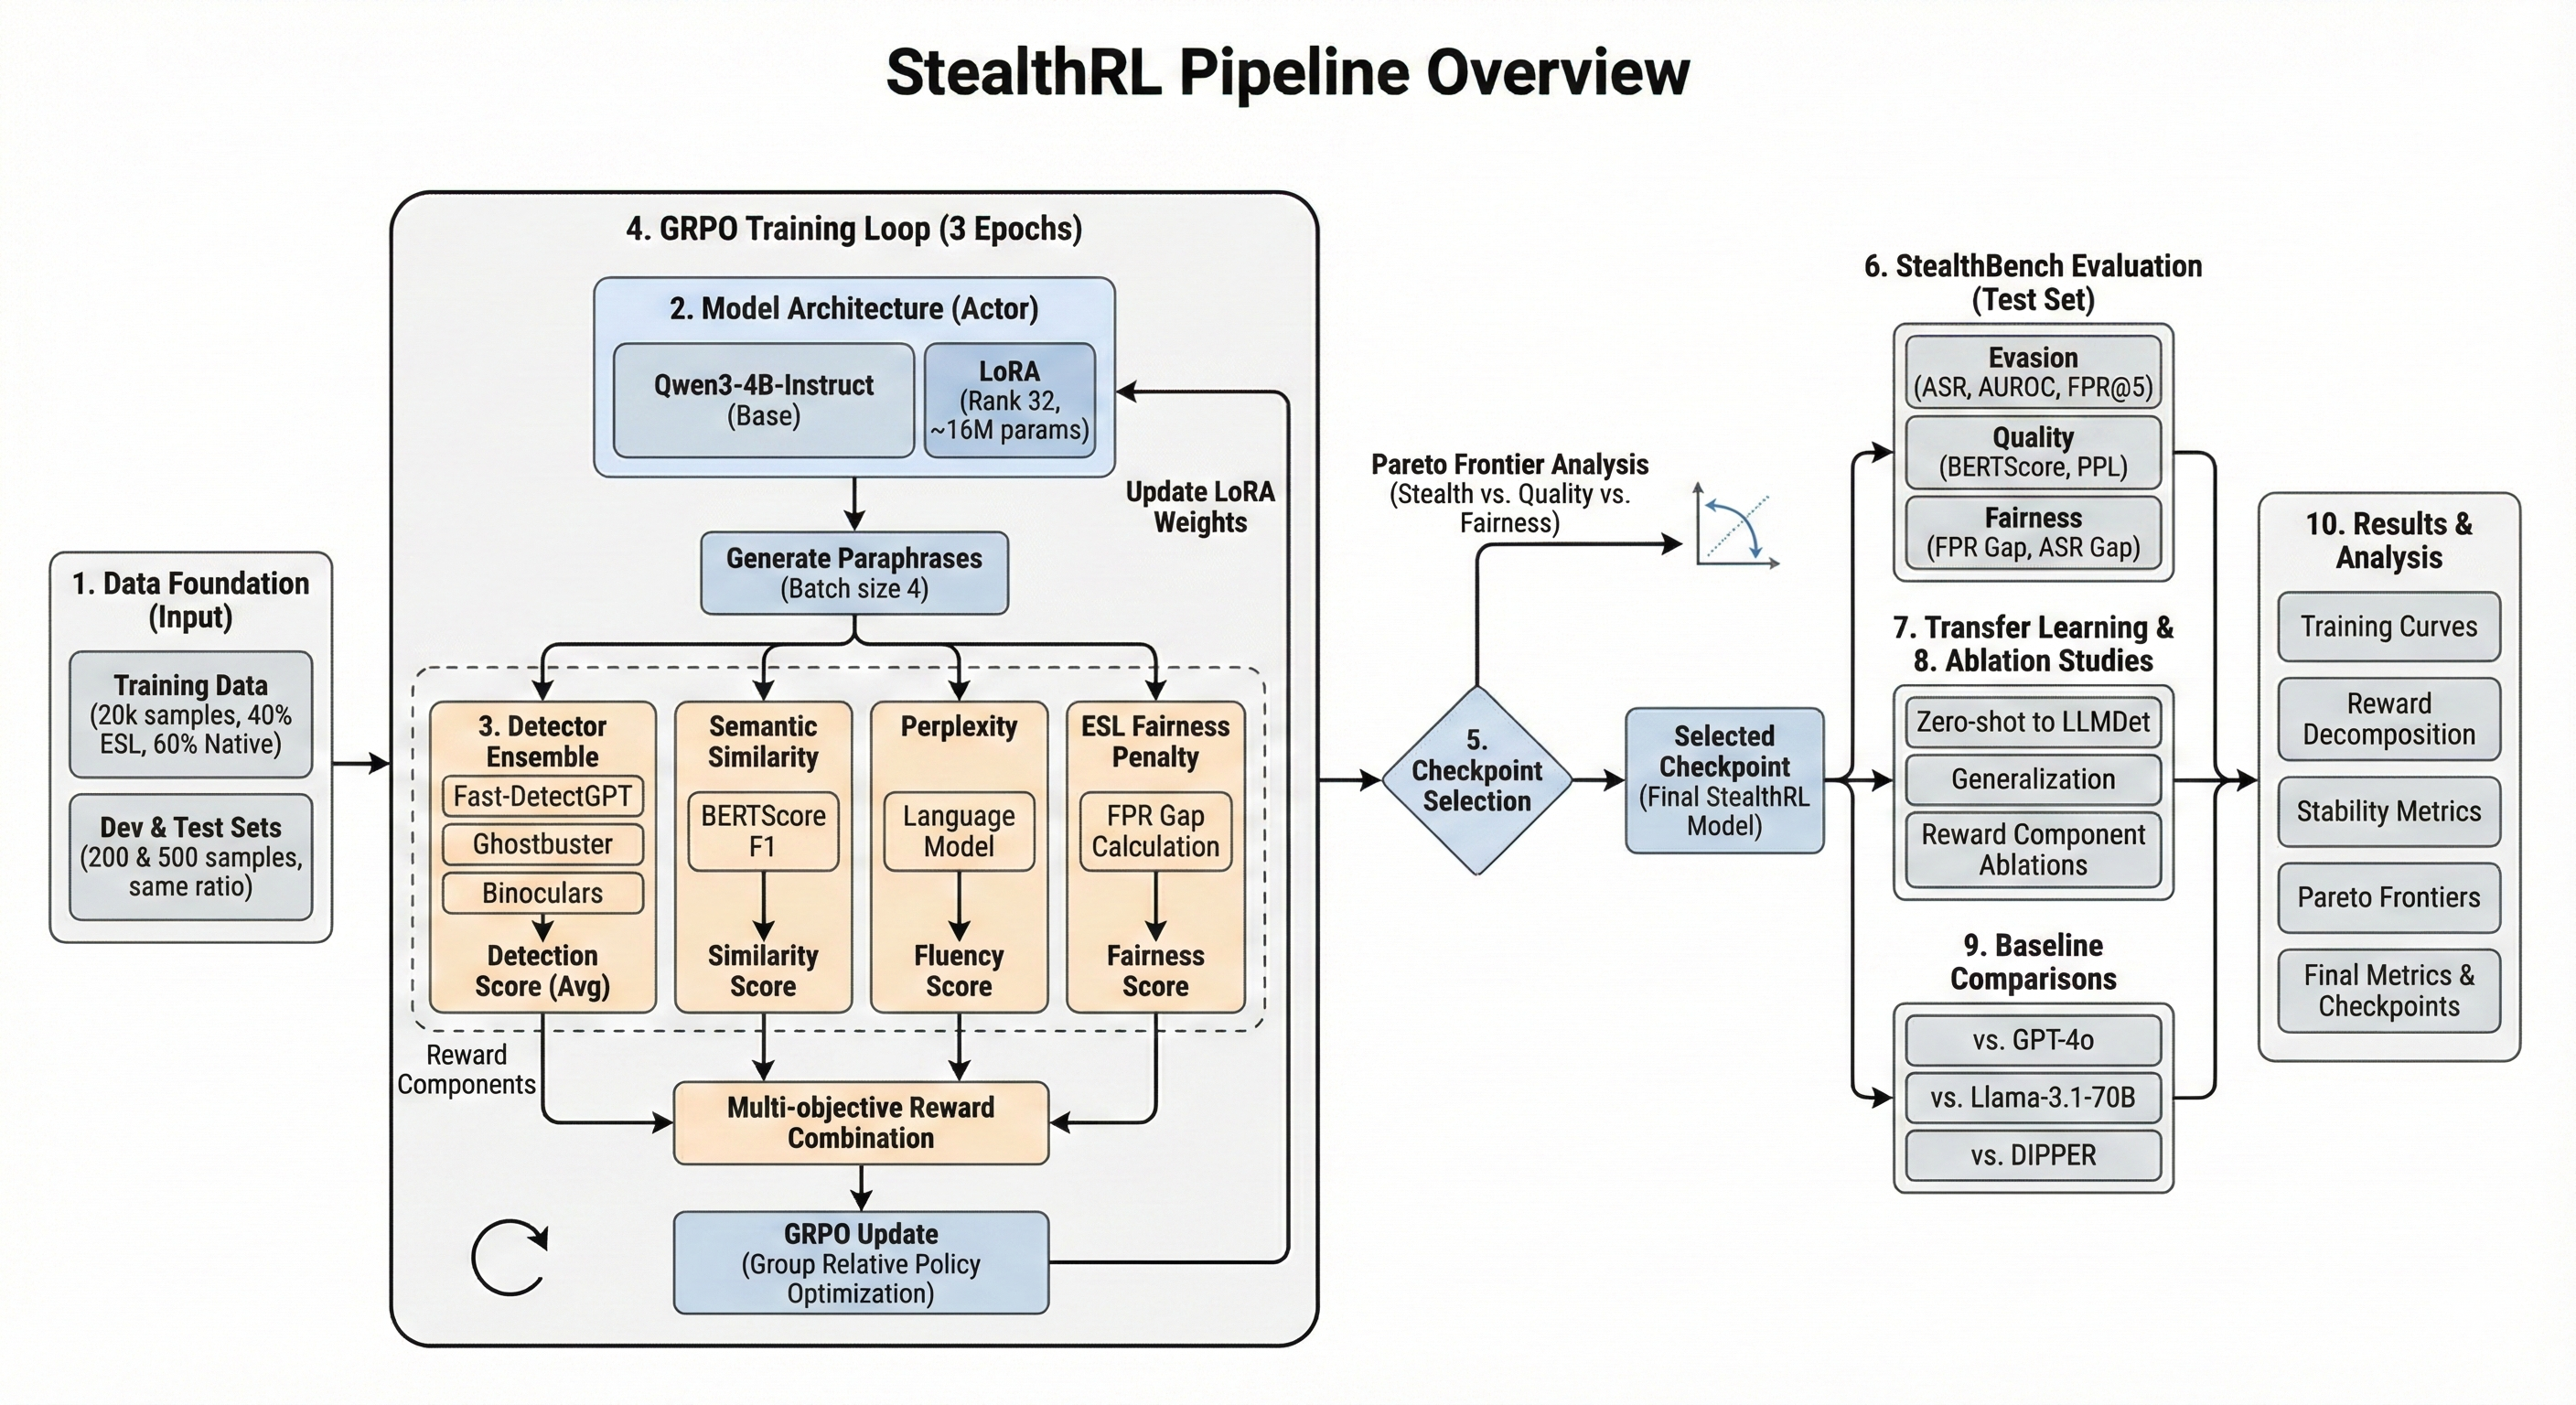
\includegraphics[width=\linewidth]{figures/StealthRL_Methodology.png}
  \caption{StealthRL training and evaluation pipeline. A single paraphrase policy is trained with detector-guided reward and quality constraints, then evaluated across multiple detector families with low-FPR metrics and tradeoff analysis.}
  \label{fig:pipeline}
\end{figure}

\section{Experimental Setup}
\paragraph{Dataset.} We evaluate on MAGE (Machine-generated Text Detection in the Wild) using the test split with 50 human and 50 AI samples, filtered to a 100--500 token window. \cite{li2024magemachinegeneratedtextdetection}

\paragraph{Detectors.} Evaluation uses three detector families: RoBERTa OpenAI classifier, Fast-DetectGPT (curvature-based), and Binoculars (paired-LM). \cite{mitchell2023detectgptzeroshotmachinegeneratedtext,bao2024fastdetectgptefficientzeroshotdetection,hans2024spottingllmsbinocularszeroshot}

\paragraph{Methods.} We compare six methods: M0 (no attack), M1 (simple paraphrase), M2 (StealthRL-v1 checkpoint), M3 (detector-guided selection inspired by Adversarial Paraphrasing), M4 (AuthorMist), and M5 (homoglyph substitution). \cite{cheng2025adversarialparaphrasinguniversalattack,david2025authormistevadingaitext,creo2025silverspeakevadingaigeneratedtext}

\paragraph{Metrics.} We calibrate a 1\% FPR threshold per detector on human texts and report TPR@1\%FPR (lower is better for the attacker), attack success rate (ASR = 1 - TPR@1\%FPR), and AUROC. We also report semantic similarity (E5 cosine) to quantify fidelity. All results use one candidate per sample (n=1) to match the current evaluation run.

\paragraph{LLM-based quality evaluation (optional).} Following Adversarial Paraphrasing, we optionally use a gpt-4o-mini autorater to score paraphrase quality and semantic equivalence on a 1--5 Likert scale, capped to a fixed number of samples per method. \cite{cheng2025adversarialparaphrasinguniversalattack,vu2024foundationalautoraters,fu2023gptscore,kim2024prometheus2}

\section{Results}
Table~\ref{tab:main} summarizes detection evasion at 1\% FPR. StealthRL reduces mean TPR@1\%FPR to 0.04 (vs. 0.27 for no attack) and improves mean AUROC from 0.71 to 0.43. Per-detector TPR@1\%FPR drops from 0.22/0.28/0.32 (M0) to 0.08/0.02/0.02 (M2) on RoBERTa/Fast-DetectGPT/Binoculars, indicating strong transfer to the held-out detector family. StealthRL maintains high semantic similarity (0.953 E5 cosine), comparable to simple paraphrasing (0.959), while substantially outperforming the detector-guided baseline (M3).

\begin{table}[t]
  \centering
  \small
  \setlength{\tabcolsep}{4pt}
  \begin{tabular}{lcccccc}
\toprule
Method & TPR@1\%FPR $\downarrow$ (R) & F (Fast) & B (Binoc) & Mean $\downarrow$ & ASR $\uparrow$ & AUROC $\downarrow$ \\
\midrule
M0 No Attack & 0.23 & 0.40 & 0.41 & 0.34 & 0.66 & 0.74 \\
M1 Simple Para & 0.10 & 0.10 & 0.04 & 0.08 & 0.92 & 0.59 \\
M2 StealthRL-v1 & \textbf{0.00} & \textbf{0.00} & \textbf{0.00} & \textbf{0.00} & \textbf{1.00} & \textbf{0.27} \\
M3 Adv. Para (guided) & 0.10 & 0.09 & 0.05 & 0.08 & 0.92 & 0.60 \\
M5 Homoglyph & \textbf{0.00} & \textbf{0.00} & \textbf{0.00} & \textbf{0.00} & \textbf{1.00} & 0.44 \\
\bottomrule
\end{tabular}

  \caption{Main results on MAGE (TPR@1\%FPR, ASR, and AUROC). Lower TPR/AUROC is better for the attacker; higher ASR is better. R/F/B denote RoBERTa/Fast-DetectGPT/Binoculars.}
  \label{tab:main}
\end{table}

\begin{figure}[t]
  \centering
  \includegraphics[width=0.92\linewidth]{figures/fig_heatmap_tpr.png}
  \caption{Detector \(\times\) method heatmap of TPR@1\%FPR. StealthRL shows consistently low TPR across detectors, indicating transfer beyond the training ensemble.}
  \label{fig:heatmap}
\end{figure}

\begin{figure}[t]
  \centering
  \includegraphics[width=0.85\linewidth]{figures/fig_tradeoff.png}
  \caption{Evasion--quality tradeoff (mean TPR@1\%FPR vs. semantic similarity). StealthRL achieves strong evasion while preserving meaning; homoglyph attacks improve evasion but degrade fluency and readability.}
  \label{fig:tradeoff}
\end{figure}

\paragraph{Ablation (implemented; results pending).} We implemented a \emph{guidance-transfer} ablation that mimics the ``guidance vs. deploy'' setting from Adversarial Paraphrasing: candidate selection is guided by (i) RoBERTa, (ii) Fast-DetectGPT, or (iii) the ensemble mean, and evaluated across all detectors. This isolates how guidance detector choice affects transfer. Results are pending for the final model checkpoints.

\section{Limitations and Safety}
Our evaluation currently focuses on three detector families and one primary benchmark; additional detectors (e.g., watermark-based) and datasets can broaden coverage. Adversarial paraphrasing is dual-use: we present StealthRL as a red-teaming tool to expose detector fragility and inform defensive calibration, and we release code anonymized with the expectation of responsible use.

\section{LLM Usage Disclosure}
Large language models were used to assist with code scaffolding and with editing text for clarity. All modeling decisions, experiments, evaluations, and interpretations were designed, executed, and validated by the authors.

\section{Conclusion}
StealthRL provides a practical adversarial RL framework for generating high-fidelity paraphrases that evade multiple detector families under strict low-FPR constraints. Our results show strong transfer to a held-out detector while preserving semantic fidelity, and our released evaluation pipeline supports reproducible red-teaming of AI-text detectors.

\bibliographystyle{iclr2026_conference}
\bibliography{stealthrl_refs}

\appendix
\section{Qualitative Examples}
\begin{table}[h]
\centering
\small
\setlength{\tabcolsep}{4pt}
\begin{tabularx}{\linewidth}{X X}
\toprule
\textbf{Original (M0)} & \textbf{StealthRL (M2)} \\
\midrule
During cardio the heart increases its workload and all the body's other systems adjust to help support that endeavor. The blood vessels dilate, the muscles do their best to help pump blood back to the heart, and the lungs work harder to take in oxygen and remove waste gases like carbon dioxide. &
In cardio, the heart ramps up its workload, prompting the body's other systems to adapt and assist. Blood vessels widen, muscles strive to push blood back to the heart, and lungs intensify their efforts to absorb oxygen and expel waste gases such as carbon dioxide. \\
\midrule
The engine has to endure the torque of powering two axels and a drive shaft generally the transfer casing connects to the drive shaft with a ujoint and same for power distribution. The electricity goes into the battery first then is sent to the alternator where it generates voltage that powers all other electrical components like the lights, radio. &
The engine must handle the torque from two axles and a drive shaft, typically linked via a universal joint in the transfer casing for power distribution. Electricity first charges the battery, then flows to the alternator, which converts it into voltage to power essential electrical systems such as lights and the radio. \\
\bottomrule
\end{tabularx}
\caption{Representative paraphrases from the evaluation run (MAGE test split).}
\end{table}
\end{document}
